\chapter{MEAN-FIELD LIMIT IN THE DETERMINISTIC SETTING}
In this chapter we focus on the deterministic version of the mean-field limit. Namely, we
start from a system of deterministic interacting particle system with mean-field structure
and prove that the corresponding empirical measure converges weakly to the measure valued solution of 
the corresponding partial differential equation. We are going to work only with the first order system, recall
\begin{Definition}[1st Order Particle System]
  We consider a system of $N$ particles and denote by $(x_{1}(t),x_{2}(t),\ldots,x_N(t)) \in  \mathcal{C}^{1}([0,T];\mathbb{R}^{d} ),\ i=1,\ldots ,N $ 
  the trajectories of the particles.\\[1ex]
  Our first order system is then governed by the system of ordinary differential equations 
  \begin{align*}
    \begin{cases}
      d x_i(t) &= \frac{1}{N}\sum_{j=1}^{N} K(x_{i},x_{j}) dt  \quad 1\le i \le N \\
        x_i(t)\rvert_{t=0} &= x_i(0) \in \mathbb{R}^{d} 
    \end{cases}
  .\end{align*}
  where $K : \mathbb{R}^{2d} \to \mathbb{R}^{d}  $ is a given function.\\[1ex]
\end{Definition}
 In the case of higher dimensional vectors we sometimes  use the following notation 
 \begin{align*}
  X_N(t) = \begin{pmatrix} x_{1}(t),x_2(t),\ldots ,x_N(t) \end{pmatrix}^{T}  \in \mathbb{R}^{dN} 
 .\end{align*}
\section{Review Of ODE Theory}
\begin{definition}[Intial Value Problem]\label{ivp}
  For $\forall T > 0$ and\\ $f\:\ [0,T] \times  \mathbb{R}^{d} \to \mathbb{R}^{d} $ we consider the initial value problem given by
  \begin{align*}
    \text{(IVP)} \begin{cases}
     \frac{d}{dt} x(t) &= f(t,x) \quad t \in  [0,T]\\
     x \rvert_{t=0} &= x_{0} \in  \mathbb{R}^d
     \end{cases}
  .\end{align*}
\end{definition}
\begin{assumption}\label{assumption_a}
  $f \in  \mathcal{C}([0,T] \times  \mathbb{R}^{d} ; \mathbb{R}^{d}  )$  and 
  $f$ is Lipschitz continuous in $x$, which means there $\exists L >0$ such that 
    $\forall (t,x),(t,y) \in  [0,T] \times \mathbb{R}^{d}$
  \begin{align*}
    &\abs{f(t,x) - f(t,y)} \le  L \abs{x-y}
  .\end{align*}
\end{assumption}
\begin{theorem}[Existence and uniqueness of IVP]\label{existence_uniqueness}
  If \autoref{assumption_a} holds then the (IVP) has a unique solution $x \in  \mathcal{C}^{1}([0,T];\mathbb{R}^{d} ) $
\end{theorem}
\begin{proof}
 We use Picard iteration to prove the existence, we can define the equivalent way of solving the (IVP) by considering the integral equation
 \begin{align*}
   x(t) - x_{0} = \int_0^{t} f(s,x(s)) ds \quad \forall t \in  [0,T]
 .\end{align*}
 Then our Picard iteration is given by the following 
 \begin{align*}
   x_1(t) &= x_{0} + \int_0^{t} f(s,x_{0})  ds \\
   x_2(t) &= x_{0} + \int_0^{t} f(s,x_{1}(s))  ds \\
          &\vdots \\
   x_m(t) &= x_{0} + \int_0^{t} f(s,x_{m-1}(s))  ds
 .\end{align*}
 By \autoref{assumption_a} and properties of integration we have $x_m(t) \in  \mathcal{C}^{1}([0,T];\mathbb{R}^{d} ) $.\\[1ex]
 Due to completeness of $\mathcal{C}^{1}([0,T];\mathbb{R}^{d} )$ we only need to show that $(x_m(t))_{m \in  \mathbb{N}}$ is a Cauchy sequence 
 to get the existence. We first prove by induction that for $m\ge 2$ it holds for some constant $M$ that
 \begin{align*}
   \abs{x_m(t) - x_{m-1}(t)} \le \frac{ML^{m-1}\abs{t}^{m}  }{m!}
 .\end{align*}
 \textbf{IA} For $m=1$ it holds 
 \begin{align*}
   \abs{x_2(t) - x_{1}(t)} &\myS{Tri.}{\le } \int_0^{t}  \abs{f(s,x_{1}(s))-f(s,x_{0})}ds\\
                           &\le L \int_0^{t} \abs{x_{1}(s_{0})-x_{0}}  ds_{0}\\
                           &\le L \int_0^{t} \int_0^{s_{0}}   \abs{f(s_{1},x_{0})}ds_{1}ds_{0}\\
                           &\le ML \int_0^{t}(s_{0}-0)  ds_{0} \\
                           &= \frac{MLt^2}{2}
 .\end{align*}
 where we chose $M \ge  \max_{s \in  [0,T]} \abs{f(s,x_{0})}$ \\
 \textbf{IV} Suppose for $m \in  \mathbb{N}$ it holds 
 \begin{align*}
   \abs{x_m(t)-x_{m-1}(t)} \le  \frac{ML^{m-1}\abs{t}^m }{m!}
 .\end{align*}
 \textbf{IS} $m \to  m+1$ 
 \begin{align*}
   \abs{x_{m+1}(t)-x_m(t)}&= \abs*{\int_0^{t} f(s,x_m(s)) - f(s,x_{m-1}(s)) ds }\\
                          &\myS{Tri.}{\le }  \int_0^{t} \abs{f(s,x_m(s))-f(s,x_{m-1})(s)} ds \\
                          &\le L \int_0^{t} \abs{x_m(s) - x_{m-1}(s)}   ds \\
                          &\myS{IV}{\le } L \int_0^{t} \frac{ML^{m-1}\abs{s}^{m}  }{m!}  ds\\
                          &= \frac{ML^{m}\abs{t}^{m+1} }{(m+1)!}
 .\end{align*}
 Now take arbitrary $p,m \in  \mathbb{N}$  then by triangle inequality we obtain for $\forall  t \in  [0,T]$ that 
 \begin{align*}
   \abs{x_{m+p} - x_{m}(t)} &\le  \sum_{k=m+1}^{m+p}  \abs{x_k(t) - x_{k-1}(t)} \\
                            &\le \sum_{k=m+1}^{m+p} M \frac{L^{k-1}T^{k}  }{k!} \\
                            &= \frac{M}{L} \sum_{k=m+1}^{m+p} \frac{(LT)^{k} }{k!}\\
 .\end{align*}
 Continuing on the next page
 \begin{align*}
  \frac{M}{L} \sum_{k=m+1}^{m+p} \frac{(LT)^{k} }{k!} &\le \frac{M}{L} \frac{(LT)^{m+1} }{(m+1)!} \sum_{k=0}^{p-1}\frac{(LT)^{k} }{k!} \\
                                                      &\le \frac{M}{L}\frac{(LT)^{m+1} }{(m+1)!}\sum_{k=0}^{\infty} \frac{(LT)^{k} }{k!} \\
                                                      &= \frac{M}{L}\frac{(LT)^{m+1} }{(m+1)!} e^{LT} \xrightarrow{m\to \infty} 0 \text{ uniformly in } t\in [0,T]
 .\end{align*}
 Therefore $x_m(t)$ has a limit $x(t) \in  \mathcal{C}^{1}([0,T];\mathbb{R}^{d} ) $ with 
 \begin{align*}
   \max_{t \in  [0,T]} \abs{x_m(t) - x(t)} \xrightarrow{m\to \infty} 0
 .\end{align*}
 Then by taking $m\to \infty$ in 
 \begin{align*}
   x_m(t) = x_{0} + \int_{t_{0}}^{t} f(s,x_{m-1}(s)) ds
 .\end{align*}
 we get 
 \begin{align*}
   x(t) = x_{0} + \int_{t_{0}}^{t} f(s,x(s)) ds
 .\end{align*}
 which means $x(t) \in  \mathcal{C}^{1}([0,T];\mathbb{R}^{d} ) $ is a solution of the equivalent integral equation.\\[1ex]
 To prove the uniqueness suppose we have two solutions $x(t),\tilde{x}(t) \in  \mathcal{C}^{1}([0,T];\mathbb{R}^{d} )  $ then they satisfy 
 \begin{align*}
   x(t) &= x_{0} + \int_{t_{0}}^{t} f(s,x(s))  ds \\
   \tilde{x}(t) &= x_{0} + \int_{t_{0}}^{t} f(s,\tilde{x}(s) )   ds
 .\end{align*}
 By taking the difference of these two solutions and using the Lipschitz continuity  of $f$ in $x$ we obtain 
 \begin{align*}
   \abs{x(t)- \tilde{x}(t) } &\le \int_0^{t} \abs{f(s,x(s)) - f(s,\tilde{x(s)} )} ds  + \abs{x_{0}-x_{0}}\\
                             &\le L\int_)^{t} \abs{x(s) - \tilde{x}(s) }   ds \\
                             &\le  L \int_{0}^{t} e^{-\alpha s}  \abs{x(s) - \tilde{x}(s) }e^{\alpha s}  ds
 .\end{align*}
 For any $\alpha >0$. By considering the quantity $P(t) = e^{-\alpha t} \abs{x(t) - \tilde{x}(t) } $, we obtain 
 \begin{align*}
   \abs{x(t) - \tilde{x}(t) } &\le L \int_0^{t} \max_{0 \le s\le t}  \{e^{-\alpha  s}\abs{x(s)-\tilde{x}(s) } \} e^{\alpha  s}    ds \\
                              &\le  L \max_{0\le s\le t} \{e^{-\alpha s}\abs{x(s)-\tilde{x}(s) } \}   \int_0^{t} e^{\alpha s}  ds
 .\end{align*}
 We obtain 
 \begin{align*}
   P(t) = e^{-\alpha t} \abs{x(t)-\tilde{x}(t) } \le \max_{t \in  [0,T]} P(t) \le  \frac{L}{\alpha } \max_{t \in  [0,T]} P(t) \quad \forall t \in [0,T]
 .\end{align*}
 By choosing $\alpha  = 2L$ we have 
 \begin{align*}
   \max_{t \in  [0,T]} e^{-2Lt}  \abs{x(t) - \tilde{x}(t) } = 0
 .\end{align*}
 i.e 
 \begin{align*}
   x(t) = \tilde{x}(t)  \quad \forall t \in [0,T]
 .\end{align*}
This concludes the uniqueness proof
\end{proof}
\begin{remark}
 An alternative proof for uniqueness uses  Gronwall's inequality
 which we give in the following. Furthermore similar to the uniqueness proof, one can 
 obtain that the solution $x(t; t_{0},x_{0})$ is continuously dependent on initial data
\end{remark}
\begin{lemma}[Gronwall's inequality]\label{gronwall_lemma}
  Let $\alpha ,\beta ,\phi  \in  \mathcal{C}([a,b];\mathbb{R}^{d} )$  and $\beta (t) \ge 0$ for $\forall t \in [a,b]$ 
  such that 
  \begin{align*}
    0 \le  \phi(t) \le  \alpha(t) + \int_a^{t} b(s)\phi(s) ds \quad \forall t \in [a,b] 
  .\end{align*}
  then 
  \begin{align*}
    \phi(t) \le  \alpha(t) + \int_a^{t}  \beta(s) e^{\int_s^{t} \beta(\tau ) d\tau  }  \alpha(s) ds \quad \forall t \in [a,b]
  .\end{align*}
  Specially if $\alpha(t) \equiv M$ then we have 
  \begin{align*}
    \phi(t) \le  M e^{\int_a^{b} \beta(\tau )d\tau  }  \quad \forall t \in [a,b]
  .\end{align*}
\end{lemma}
\begin{proof}
 Define 
 \begin{align*}
   \psi   (t) = \int_a^{t} \beta(\tau ) \phi(\tau ) d\tau  \quad \forall t \in [a,b]
 .\end{align*}
 because of the continuity of $\beta $ and $\phi $ we get that $\psi $ is differentiable on $[a,b]$ and
 \begin{align*}
  \psi'(t) = \beta(t)\phi(t)
 .\end{align*}
 Since $\beta(t) \ge $ we have 
 \begin{align*}
   \psi'(t) = \beta(t) \phi(t) \le \beta(t) (\alpha(t)+\psi(t)) \quad \forall t \in [a,b]
 .\end{align*}
 Then by multiplying both sides with $e^{-\int_a^{t} \beta(\tau ) d\tau  } $ we obtain 
 \begin{align*}
   \frac{d}{dt} (e^{-\int_a^{t} \beta(\tau ) d\tau  }\psi(t) ) &= e^{-\int_a^{t} \beta(\tau ) d\tau  }(\psi'(t) - \beta(t)\psi(t))\\
                                                               &\le \beta(t)\alpha(t)e^{-\int_a^{t} \beta(\tau ) d\tau  }
 .\end{align*}
 Integrate the above inequality from  $a$ to $t$ to get 
 \begin{align*}
  e^{-\int_a^{t} \beta(\tau ) d\tau  }\psi(t) - e^{-\int_a^{t} \beta(\tau ) d\tau  }\psi (a) \le \int_a^{t} \beta(s)\alpha(s) e^{-\int_a^{s} \beta(\tau ) d\tau  }  ds
 .\end{align*}
 Which implies 
 \begin{align*}
  \psi(t) \le \int_a^{t} \beta(s)\alpha(s)  e^{\int_s^{t} \beta(\tau ) d\tau  } ds
 .\end{align*}
 and 
 \begin{align*}
  \phi(t) \le \alpha(t) + \psi(t) \le  \alpha(t) + \int_a^{t} \beta(s) \alpha(s)e^{\int_s^{t} \beta(\tau ) d\tau  }  ds
 .\end{align*}
 The case with $\alpha(t) \equiv M$ is handled by using the main theorem of Differential and Integral calculus 
 \begin{align*}
   \phi(t) &\le  M \left( 1+\int_a^{t} \beta(s) e^{\int_s^{t}\beta(\tau )d\tau  } ds   \right) \\
           &= M(1-e^{\int_s^{t} \beta(\tau ) d\tau  }\rvert_a^{t}  ) \\
           &= Me^{\int_a^{t}\beta(\tau ) d\tau  } 
 .\end{align*}
\end{proof}
\newpage
\section{Mean-field particle system, well-posedness and problem setting}
Let us again give the model and problem setting
\begin{definition}[1st Order Particle System]\label{first_order_system}
  We consider a system of $N$ particles and denote by $(x_{1}(t),x_{2}(t),\ldots,x_N(t)) \in  \mathcal{C}^{1}([0,T];\mathbb{R}^{d} ),\ i=1,\ldots ,N $ 
  the trajectories of the particles.\\[1ex]
  Our first order system is then governed by the system of ordinary differential equations 
  \begin{align*}
    \text{(MPS)}\begin{cases}
      d x_i(t) &= \frac{1}{N}\sum_{j=1}^{N} K(x_{i},x_{j}) dt  \quad 1\le i \le N \\
        x_i(t)\rvert_{t=0} &= x_i(0) \in \mathbb{R}^{d} 
    \end{cases}
  .\end{align*}
  where $K : \mathbb{R}^{2d} \to \mathbb{R}^{d}  $ is anti-symmetric i.e
  \begin{align*}
    K(x,y) = -K(y,x) \quad K(x,x) = 0
  .\end{align*}
\end{definition}
\begin{assumption}\label{assumption_b}
  $K \in  \mathcal{C}^{1}(\mathbb{R}^{d} \times \mathbb{R}^{d} ; \mathbb{R}^{d}   ) $ and there exists some $L>0$ such that
  $\forall x,y \in \mathbb{R}^{d} $ it holds 
  \begin{align*}
    \sup_y \abs{\nabla_x K(x,y)} + \sup_x \abs{\nabla_yK(x,y)} \le L
  .\end{align*}
\end{assumption}
\begin{lemma}
  When \autoref{assumption_b} holds for $K$ then for $\forall T>0$ the (MPS) has a unique solution 
  \begin{align*}
    X_N(t) = (x_{1}(t),x_{2}(t),\ldots ,x_{N}(t)) \in  \mathcal{C}^{1} ([0,T];\mathbb{R}^{dN} )
  .\end{align*}
  and for any fixed $t \in  [0,T]$ the map
  \begin{align*}
    X_N(t,*): \mathbb{R}^{dN} \to \mathbb{R}^{dN}  \ :\ x \mapsto X_N(t,x)
  \end{align*}
  is a bijection 
\end{lemma}
In the introduction we saw that the empirical measure satisfies a partial differential equation
\begin{definition}[PDE Problem]
  Let $\mu ^{N}(t) $ be the empirical measure 
  \begin{align*}
    \mu ^{N }(t) \triangleq \frac{1}{N}  \sum_{j=1}^{N} \delta_{x_i(t)} 
  .\end{align*}
Then from the introduction we know that for $\forall \phi  \in \mathcal{C}_0^{\infty}(\mathbb{R}^{d} ) $  the empirical measure satisfies
\begin{align*}
  \frac{d}{dt} \braket{\mu^N(t),\phi } = \braket{\mu^N(t),\nabla \phi *\mathcal{K}\mu ^{N}(t) }
.\end{align*}
where 
\begin{align*}
  \mathcal{K}\mu ^{N}(*) = \int_{\mathbb{R}^{d} }  K(*,y) d\mu ^{N}(y) 
.\end{align*}
\end{definition}
\begin{idea}
 If $\mu ^{N} \to \mu  $  in some sense, then the limiting measure $\mu $ should also satisfy 
 \begin{align*}
  \begin{cases}
    &\partial_t \mu  + \nabla * (\mu \mathcal{K} \mu ) = 0 \\
    & \mu^N(0)   \to \mu_0
  \end{cases}
 .\end{align*}
 in the sense weak sense i.e. the "sense of distributions" which we define in the following section
\end{idea}
\section{A short introduction for Distributions}
\begin{definition}
 Let $\Omega  \subset  \mathbb{R}^{d} $  be an open subset then the space of test functions $\mathcal{D}(\Omega )$
 consists of all the functions in $\mathcal{C}_0^{\infty}(\Omega ) $ supplemented by the following convergence \\[1ex]
 We say $\phi_m \to  \phi \in  \mathcal{C}_0^{\infty}(\Omega ) $ iff 
 \begin{enumerate}
   \item There exists a compact set $\exists K \subset  \Omega $ such that $\supp \phi_m \subset  K$ for $\forall m$
   \item For all multi indices $\alpha $ it holds 
     \begin{align*}
       \sup_K \abs{\partial ^{\alpha } \phi_m - \partial ^{\alpha } \phi   } \xrightarrow{m\to \infty}  0 
     .\end{align*}
 \end{enumerate}
\end{definition}
\begin{remark}
 $\mathcal{D}(\Omega )$  is a linear space
\end{remark}
\begin{definition}[Multi-Index]
A multi-index $\alpha \in \N_0^n$ of length $\abs{\alpha } = \sum_{i} \alpha_i$
for example $\alpha  = (0,2,1) \in \N^3_0$  can be used to denote partial derivatives of higher order as such : 
\begin{align*}
  \partial^{\alpha } = \prod_i (\frac{\partial}{\partial x_i})^{\alpha_i}
.\end{align*}
\end{definition}
\begin{definition}[Distribution]
 The space of Distributions is denoted by $\mathcal{D}'(\Omega )$  and is the dual space of $\mathcal{D}(\Omega)$
 i.e. it is the linear space of all continuous linear functions on $\mathcal{D}(\Omega )$ \\[1ex]
 We say a functional $T :\mathcal{D}(\Omega ) \to \mathbb{C}$ is continuous linear iff 
 \begin{enumerate}
   \item $\braket{T,\alpha \phi_1+ \beta \phi_2} = \alpha \braket{T,\phi_1} + \beta \braket{T,\phi_2}$ 
   \item If $\phi_m \to  \phi $ in $\mathcal{D}(\Omega )$ then $\braket{T,\phi_m} \to \braket{T,\phi }$
 \end{enumerate}
\end{definition}
We can define several operations on the space of distributions but since most of them are not used in this Lecture 
we only define the multiplication with a smooth function 
\begin{definition}
For a smooth function $f \in  \mathcal{C}^{\infty} $ and a distribution $T \in \mathcal{D}'$ the product is defined as follows 
\begin{align*}
  \braket{Tf,\phi } = \braket{T,f \phi} \quad \forall \phi  \in  \mathcal{D}
.\end{align*}
\end{definition}
\begin{remark}
 Multiplication between two Distributions $T,F \in  \mathcal{D}'$ is not well defined, 
 instead the convolution of two Distributions is defined 
\end{remark}
\begin{example}
  For functions $f \in  L^{1}_{\text{loc}}(\Omega ) $  we can define the associated distribution $T_f \in  \mathcal{D}'(\Omega )$ is defined by 
  \begin{align*}
    \braket{T_f,\phi } = \int_\Omega  f(x)\phi(x) dx \quad \forall \phi  \in \mathcal{D}(\Omega )
  .\end{align*}
  and say $L_{\text{loc}}^{1}(\Omega ) \subset \mathcal{D}'(\Omega )  $\\[1ex]
  Similarly $L^{p}_{\text{loc}} \subset  \mathcal{D}'(\Omega ) $, using Hölder's inequality one obtains
  $L_{\text{loc}}^{p}(\Omega ) \subset L_{\text{loc}}^{q}(\Omega )   $ for $1<q<p<\infty$
\end{example}
\begin{remark}
 The support of a distribution is also well-defined 
\end{remark}
\begin{theorem}
  $L^{1}_{\text{loc}} $ functions are uniquely deterimed by distributions. More precisely 
  for two functions $f,g \in  L_{\text{loc}}^{1}(\Omega ) $  if 
  \begin{align*}
    \int_\Omega  f \phi dx = \int_\Omega  g \phi dx \quad \forall \phi  \in \mathcal{D}(\Omega )
  .\end{align*}
  then $f = g$ a.e. in $\Omega $
\end{theorem}
\begin{proof}
 This proof is left as an exercise  
\end{proof}
\begin{example}
 The set of probability density functions on $\mathbb{R}$ is a subset of $\mathcal{D}'(\mathbb{R} )$.
 For any probability density function $P(x)$ the associated distribution  $T_P \in \mathcal{D}'(\mathbb{R})$
 is defined by
 \begin{align*}
   \braket{T_P,\phi } = \int_\mathbb{R} \phi(x) P(x) dx \quad \forall  \phi  \in \mathcal{D}(\mathbb{R})
 .\end{align*}
\end{example}
\begin{example}
 The set of  measures  $\mathcal{M}(\Omega )$ is a subset of $\mathcal{D}'(\Omega )$. 
 For any $\mu \in \mathcal{M}(\Omega )$ the associated distribution $T_{\mu }$ is defined by 
 \begin{align*}
   \braket{T_\mu ,\phi } = \int_\Omega \phi(x) d\mu  \quad \forall \phi  \in \mathcal{D}(\Omega )
 .\end{align*}
\end{example}
\begin{example}
 An important example of a distribution which is not defined in the above way
 is the Delta distribution $\delta_y(x)$  (concentrated on $y \in  \mathbb{R}^{d} $) 
 \begin{align*}
   \braket{\delta_y,\phi } = \int_{\mathbb{R}^{d} } \phi(x) d \delta_y(x) = \phi(y) \quad \forall \phi  \in \mathcal{D}(\Omega )
 .\end{align*}
 where 
 \begin{align*}
  \delta_y(E) = \begin{cases}
    1, &y \in  E \\
    0,&y \notin E
  \end{cases}
 .\end{align*}
\end{example}
The empirical measure $\mu ^{N} $ is actually given by using the Delta distribution 
\begin{align*}
  \mu ^{N}(t) \triangleq \frac{1}{N} \sum_{j=1}^{N} \delta_{x_i(t)}   \quad \braket{\mu ^{N},\phi  } = \frac{1}{N} \sum_{j=1}^{N} \phi(x_i(t)) 
.\end{align*}
We define the convergence for a sequence of distributions as follows 
\begin{definition}
  For a sequence of distributions $(T_m)_{m \in  \mathbb{N}} \subset  \mathcal{D}'(\Omega )$  we was it converges against
  a limit $T \in \mathcal{D}'(\Omega )$ iff 
  \begin{align*}
    \braket {T_m,\phi } \to \braket{T,\phi } \quad \forall \phi  \in \mathcal{D}(\Omega )
  .\end{align*}
\end{definition}
Based on this convergence we give some examples in the approximation of $\delta_0(x)$
\begin{example}[Heat Kernel]
 The heat kernel for $x \in  \mathbb{R}$ and $t>0$ is given by
 \begin{align*}
   f_t(x) = \frac{1}{(4\pi t)^{\frac{1}{2}}} e^{-\frac{\abs{x}^2}{4t}} 
 .\end{align*}
\begin{figure}[H]
  \begin{center}
    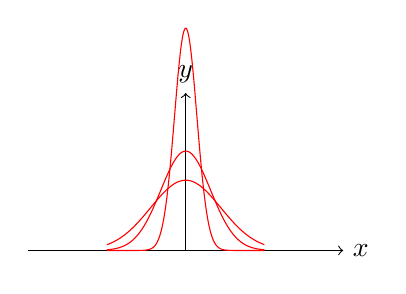
\begin{tikzpicture}
% Axes
\draw[->] (-2,0) -- (2,0) node[right] {$x$};
\draw[->] (0,0) -- (0,2) node[above] {$y$};
% Heat kernel for t = 0.1
\draw[red, domain=-1:1, samples=500] plot (\x, {1/(2*sqrt(pi * 0.1))*exp(-\x*\x/(0.1*4))});
\draw[red, domain=-1:1, samples=500] plot (\x, {1/(2*sqrt(pi * 0.05))*exp(-\x*\x/(0.05*4))});
\draw[red, domain=-1:1, samples=500] plot (\x, {1/(2*sqrt(pi * 0.01))*exp(-\x*\x/(0.01*4))});
% \draw[red, domain=-4:4, samples=100] plot (\x, {1.8*exp(-\x*\x/(0.1*4))});
\end{tikzpicture} 
  \end{center}
  \caption{Heat Kernel for different $t$}
\end{figure}
\end{example}
\begin{lemma}
  The sequence of distributions associated to the heat kernel converge to the Delta distribution 
\end{lemma}
\begin{proof}
 We consider the limit $t\to 0^+$  and obtain $\forall \phi  \in  \mathcal{C}_0^{\infty}(\Omega ) $
 \begin{align*}
   \lim_{t \to 0^+} \int_\mathbb{R} f_t(x) \phi(x) &= \lim_{t \to  0^+} \int_\mathbb{R} \frac{1}{(4\pi t)^{\frac{1}{2}} } e^{-\frac{\abs{x}^2}{4t}} \phi(x)\\
                                                   &= \lim_{t \to 0^+} \int_{-\infty}^{\infty} \frac{1}{\sqrt{\pi} }  e^{-y^2}  \phi(2 \sqrt{t}y) dy \\
                                                   &= \phi(0) = \braket{\delta_0,\phi }
 .\end{align*}
 where we used $x = 2\sqrt{t}y $ 
\end{proof}
\begin{example}
  For the rectangular functions 
  \begin{align*}
    Q_n(x) = \begin{cases}
      \frac{n}{2} ,&\abs{x} \le \frac{1}{n}\\
      0,&\abs{x} >\frac{1}{n}
    \end{cases}
  .\end{align*}
  Then
  \begin{align*}
    Q_n \xrightarrow{n\to \infty} \delta_0(x)
  .\end{align*}

\begin{figure}[H]
  \begin{center}
    \begin{tikzpicture}
% Axes
\draw[->] (-2,0) -- (2,0) node[right] {$x$};
\draw[->] (0,0) -- (0,2) node[above] {$y$};
\draw[red] (-1,0)  -- (-1,1) -- (1,1) -- (1,0);
\draw[red] (-0.5,0)  -- (-0.5,2) -- (0.5,2) -- (0.5,0);
\draw[red] (-0.25,0)  -- (-0.25,3) -- (0.25,3) -- (0.25,0);
% \draw[red, domain=-4:4, samples=100] plot (\x, {1.8*exp(-\x*\x/(0.1*4))});
\end{tikzpicture} 
  \end{center}
  \caption{Rectangular functions for different $n$}
\end{figure}
\end{example}
\newpage
\begin{example}
 The Dirichlet kernel 
 \begin{align*}
  D_n(x) = \frac{\sin(n+\frac{1}{2})x}{\sin \frac{x}{2}} = 1+2 \sum_{k=1}^{n} \cos(kx) 
 .\end{align*}
 Then 
 \begin{align*}
   D_n \xrightarrow{n\to \infty}2\pi \delta_0(x)
 .\end{align*}
\begin{figure}[H]
  \begin{center}
    
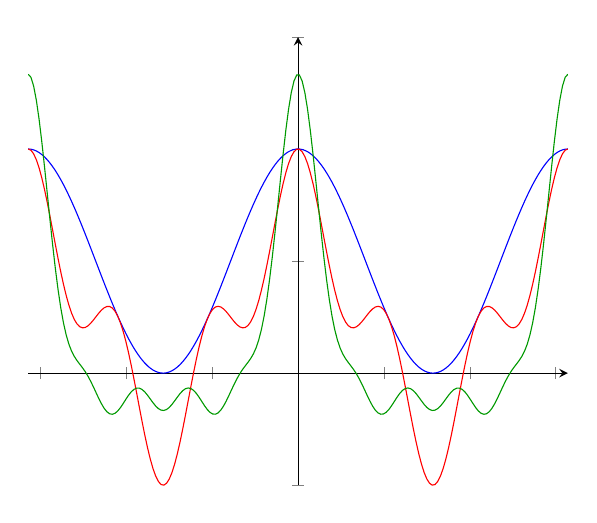
\begin{tikzpicture}
\begin{axis}[
    domain=-2*pi:2*pi,
    samples=200,
    axis lines=center,
    xlabel style={below right},
    ylabel style={above left},
    yticklabels={,,},
    xticklabels={,,},
    xmin=-2*pi,
    xmax=2*pi,
    ymin=-0.5,
    ymax=1.5,
]
% n = 1
\addplot[blue] {1/2 + (1/2)*cos(deg(x))};
% n = 3
\addplot[red] {1/4 + (1/2)*cos(deg(x)) + (1/4)*cos(3*deg(x))};
% n = 5
\addplot[green!60!black] {1/6 + (1/2)*cos(deg(x)) + (1/3)*cos(2*deg(x)) + (1/6)*cos(3*deg(x)) + (1/12)*cos(4*deg(x)) + (1/12)*cos(5*deg(x))};
\end{axis}
\end{tikzpicture}  
\end{center}
\caption{Dirichlet kernel for different $n$}
\end{figure}
\end{example}
\section{Weak Derivative Of Distributions}
\begin{definition}
 For all distributions  $\forall  T \in  \mathcal{D}'(\Omega )$  we define the derivative $\partial_i T$ by 
 \begin{align*}
   \braket{\partial_i T,\phi } &\coloneqq -\braket{T,\partial_i \phi } \quad \forall \phi  \in \mathcal{D}(\Omega)
   \braket{\partial_i^{\alpha }  T,\phi } &\coloneqq (-1)^{\abs{\alpha }} \braket{T,\partial_i^{\alpha }  \phi } \quad \forall \phi  \in \mathcal{D}(\Omega)
 .\end{align*}
 For multi index $\alpha $ 
\end{definition}
\begin{exercise}
  Prove the function $-\braket{T,\partial_i \phi }$  is a continuous and linear function  \\[1ex]
  \textit{Hint:} Consider the case where $T \coloneqq T_f$ for $f \in  L_{\text{loc}}^{1} $
\end{exercise}
We give a couple examples 
\begin{example}
 For  $\forall \phi  \in  \mathcal{D}(\Omega )$ the weak derivative of the Dirac Delta distribution is given by 
 \begin{align*}
   \braket{\delta'_0,\phi } &= - \braket{\delta_0,\phi'} = -\phi(0)\\
   \braket{\delta_0^{(k)},\phi  } &= (-1)^{k} \phi ^{(k)}  (0)
 .\end{align*}
\end{example}
\begin{lemma}
 The weak derivative of the $1$-D Heaviside function 
 \begin{align*}
  H(x) = \begin{cases}
    1, &x\ge 0,\\
    0,&x<0
  \end{cases}
 .\end{align*}
 is the Dirac Delta distribution
\end{lemma}
\begin{proof}
 For $\forall  \phi  \in \mathcal{D}(\Omega )$  it holds 
 \begin{align*}
   \braket{H',\phi } &\myS{Def.}{=} -\braket{H,\phi'}\\
                     &= - \int_{-\infty}^{\infty} H(x)\phi'(x)  dx \\
                     &= - \int_0^{\infty} \phi'(x) dx \\
                     &= \phi(0) \\
                     &= \braket{\delta_0,\phi }
 .\end{align*}
 Therefore 
 \begin{align*}
  H' = \delta_0
 .\end{align*}
\end{proof}
We can now go on to properly formulate the mean field partial differential equation in a weak sense
\section{Weak Formulation Of The Mean Field Partial Differential Equation}
Using the notation of the empirical measure we can rewrite our earlier definition of the (MPS) as follows
\begin{align*}
  \begin{cases}
    \frac{d}{dt} x_i(t) &= \braket{K(x_i,*),\mu^N(t,*)} = \int_{\mathbb{R}^{d} } K(x_{i},y) d\mu ^{N} (t,y)\\
    x_i(0)&=x_{i,0} \in \mathbb{R}^{d} , t \in [0,T]
  \end{cases}
.\end{align*}
As has been discussed before, the empirical measure satisfies for $\forall  \phi  \in \mathcal{C}_0^{\infty}(\mathbb{R}^{D} ) $ 
\begin{align*}
  \frac{d}{dt} \braket{\mu ^{N},\phi  } = \braket{\mu ^{N}\mathcal{K}\mu ^{N},\nabla \phi   } = \braket{- \divergence(\mu^N \mathcal{K} \mu ^{N} ),\phi }
.\end{align*}
where 
\begin{align*}
  \mathcal{K}\mu ^{N}(x) = \int_{\mathbb{R}^{d} }  K(x,y) d\mu ^{N} (y)
,\end{align*}
which means that the empirical measure $\mu ^{N} $ satisfies the following equation in the 
sense of distribution 
\begin{align*}
  \text{(MPDE)} \quad \partial_t \mu ^{N}  + \divergence(\mu ^{N}\mathcal{K}\mu ^{N}  ) = 0
.\end{align*}
\begin{exercise}
 Show $\mu ^{N}\mathcal{K}\mu ^{N}  $  is a distribution for smooth $K(x,y)$ 
\end{exercise}
Next we concentrate on the following PDE 
\begin{definition}[Mean Field Equation (MFE)]\label{mfe}
 Define the mean field equation as 
 \begin{align*}
  \text{(MFE)}\begin{cases}
    \partial_t + \divergence (\mu \mathcal{K}\mu ) &= 0\\
    \mu \rvert_{t=0} &= \mu_0
  \end{cases}
 .\end{align*}
 where
\begin{align*}
  \mathcal{K}\mu ^{N}(x) = \int_{\mathbb{R}^{d} }  K(x,y) d\mu ^{N} (y)
,\end{align*}
\end{definition}
We give the definition of the weak solution of (MFE)
\begin{definition}[Weak Solution of MFE]\label{weak_solution_of_mfe}
  For all $t \in [0,T]$ , $\mu (t) \in  \mathcal{M}(\mathbb{R}^{d} )$ is called a 
  weak solution of (MFE), where $\mathcal{M}(\mathbb{R}^{d} )$ denotes the space of measures on $\mathbb{R}^{d} $\\[1ex]
  For $\forall  \phi  \in  \mathcal{C}_0^{\infty}(\mathbb{R}^{d} ) $ it holds 
  \begin{align*}
    \braket{\mu(t),\phi } - \braket{\mu_0,\phi } = \int_0^{t} \braket{\mu (s)\mathcal{K}\mu(s),\nabla \phi } 
  .\end{align*}
\end{definition}
\begin{remark}
 If $\mu_0 =  \mu ^{N}(0) $  i.e. the initial data is given by an empirical measure, then 
 $\mu ^{N}(t,*) $ is a weak solution of the (MFE)
\end{remark}
We define the following initial value problem, the so called characteristics equation
\begin{definition}[Push Forwad Measure]
 For a measurable function $X$ and a measure $\mu_0 \in  \mathcal{M}(\mathbb{R}^{d} )$ 
 denote the push forward measure for any Borel set $B \subset \mathbb{R}^{d} $ by
 \begin{align*}
  X \# \mu_0  \coloneqq  \mu_0(X^{-1}(B) ) 
 .\end{align*}
\end{definition}
\begin{definition}[Characteristics equation]\label{characteristics_equation}
  \begin{align*}
    \begin{cases}
      \frac{d}{dt} x(t,x_{0},\mu_0) &= \int_{\mathbb{R}^{d} } K(x(t,x_{0},\mu_0),y)d\mu(y,t)\\
      x(0,x_{0},\mu_{0} )&=x_{0} \quad \forall  x_{0} \in  \mathbb{R}^{d} \\ 
      \mu(*,t) &= x(t,*,\mu_0) \# \mu_0
    \end{cases}
  .\end{align*}
  The solution flow $x(t,*,\mu_0)$ gives for any time $t>0$ a map 
  \begin{align*}
    x(t,*,\mu_0) \ : \ \mathbb{R}^{d} \to  \mathbb{R}^{d} 
  .\end{align*}
\end{definition}
\begin{remark}
  It can be easily checked that the push forward measure $\mu(t)$ obtained in the \nameref{characteristics_equation} is a 
 weak solution of the (MFE)
\end{remark}
\begin{remark}
  The solution space  of the \nameref{characteristics_equation} is  given by 
  \begin{align*}
    \mathcal{P}_1(\mathbb{R}^{d} ) = \{\mu \in \mathcal{P}(\mathbb{R}^{d} ) \ : \ \int_{\mathbb{R}^{d} } \abs{x} d \mu(x) <\infty\}  
  .\end{align*}
  where $\mathcal{P}(\mathbb{R}^{d} )$ is the space of all probability measures
\end{remark}
\begin{assumption}[Regularity]\label{regularity}
 We say an interaction force $K$ is regular if $K \in  \mathcal{C}^{1}(\mathbb{R}^{d} \times  \mathbb{R}^{d} ; \mathbb{R}^{d}   ) $ and there exists
 an $L > 0$ such that 
 \begin{align*}
   \sup_{y} \abs{\nabla_x K(x,y)} + \sup_{x} \abs{\nabla_y K(x,y)} \le L
 .\end{align*}
\end{assumption}
Actually this assumption has already been used in order to show the well-posedness of the particle system
\newpage
\begin{theorem}[Existence and Uniqueness of Characteristics Equation]\label{existence_uniqueness_char}
  Let \autoref{regularity} hold for K and $\mu_0 \in \mathcal{P}_1(\mathbb{R}^{d} )$ then the 
  \nameref{characteristics_equation}  has a unique solution $x(t,x_{0},\mu_0) \in  \mathcal{C}^{1}(\mathbb{R};\mathbb{R}^{d}  ) $
  and $x(t,*,\mu_0) \# \mu_0 \in  \mathcal{P}_1 $ for $\forall t > 0$
\end{theorem}
\begin{proof}
  The proof is based on Picard iteration. \\[1ex] 
  Let $C_1 = \int_{\mathbb{R}^{d} } \abs{x} d\mu_0(x)$ and define the following Banach space 
  \begin{align*}
    X \coloneqq  \{v \in  \mathcal{C}(\mathbb{R}^{d}) \: \ \|v\|_{X} < \infty\}  
  .\end{align*}
  Where 
  \begin{align*}
    \|v\|_X \coloneqq \sup_{x \in  \mathbb{R}^{d} } \frac{\abs{v(x)}}{1+\abs{x}}
  .\end{align*}
  As preparations we need the following estimates for the nonlocal term, by using \autoref{regularity} for $K$
  we have for $\forall  v , w \in  X$ 
  \begin{align*}
    &\abs*{\int_{\mathbb{R}^{d} }K(v(x),v(y)) d\mu_0(y) - \int_{\mathbb{R}^{d} }K(w(x),w(y)) d\mu_0(y)}\\
    &\le L \int_{\mathbb{R}^{d} } \abs{v(x)-w(x)} + \abs{v(y) - w(y)} d\mu_0(y)\\
    &\le  L \|v-w\|_{X}(1+\abs{x}) + L \|v-w\|_{X} \int_{\mathbb{R}^{d} } (1+\abs{y}) d\mu_0(y) \\
    &\le  L(2+C_{1})\|v - w\|_X (1+\abs{x})
  .\end{align*}
  Now define the Picard iteration for $\forall  y \in  \mathbb{R}^{d} $
  \begin{align*}
    x_0(t,y) &= y \\
    x_1(t,y) &= y + \int_0^{t} \int_{\mathbb{R}^{d}} K(x_{0}(s,y),x_0(s,z))d\mu_0(z)ds\\
             &\vdots \\
    x_m(t,y) &= y + \int_0^{t} \int_{\mathbb{R}^{d}} K(x_{m-1}(s,y),x_{m-1}(s,z))d\mu_0(z)ds\\
  .\end{align*}
  Then we can bound the difference between $x_{1}$ and $x_{0}$ by 
  \begin{align*}
    \abs{x_1(t,y) - x_{0}(t,y)} &= \abs*{\int_0^{t} \int_{\mathbb{R}^{d} }  K(x_{0}(s,y),x_{0}(s,z)) d\mu_0(z) ds} \\
                                &= \abs*{\int_0^{t} \int_{\mathbb{R}^{d} } K(y,z) d\mu_0(z) ds}\\
                                &\le \int_0^{\abs{t}}  \int_{\mathbb{R}^{d} }L(\abs{y} + \abs{z}) d\mu_0(z)ds\\
                                &= \int_0^{\abs{t}}  L(\abs{y} + C_1) ds \\
                                &\le L(1+C_{1})(1+\abs{y})\abs{t}
  .\end{align*}
  Furthermore for $\forall m\ge 1$ we have 
  \begin{align*}
    &\abs{x_m(t,y) - x_{m-1}(t,y)} \\
    &= \abs*{\int_0^{t} \int_{\mathbb{R}^{d} }\left( K(x_{m-1}(s,y),x_{m-1}(s,z)) - K(x_{m-2}(s,y),x_{m-2}(s,z)) \right)d\mu_0(z)ds  }\\
    &\le L(2+C_{1})\int_0^{\abs{t}} \|x_{m-1}(s,*)-x_{m-2}(s,*)\|_X(1+\abs{y}) ds
  .\end{align*}
  hence by dividing both sides by $1 + \abs{y}$ we have 
  \begin{align*}
    \|x_m(t,*) - x_{m-1}(t,*)\|_X &\le L(2+C_{1})\int_0^{\abs{t}}  \|x_{m-1}(s,*) - x_{m-2}(s,*)\|_X ds\\
                                  &\le \frac{((2+C_{1})L \abs{t})^{d} }{(m-1)!}
  .\end{align*}
  which implies for $\forall m > n \to \infty$ 
  \begin{align*}
    \|x_m(t,*) - x_n(t,*)\|_X \le  \sum_{i=n}^{m-1} \|x_{i+1}(t,*) - x_i(t,*)\|_X \to  0
  .\end{align*}
  Therefore for $T > 0 $ 
  \begin{align*}
    x_m(t,*) \to x(t,*) \text{ in } X \text{ uniformly in } [-T,T]
  .\end{align*}
  and $x \in  \mathcal{C}(\mathbb{R};\mathbb{R}^{d}  )$ satisfies that, after taking the limit in Picard iteration $\forall y \in  \mathbb{R}^{d} $
  \begin{align*}
    x(t,y) = y + \int_0^{t} \int_{\mathbb{R}^{d} } K(x(s,y),x(s,z)) d\mu_0(z) ds
  .\end{align*}
  By the fundamental theorem of calculus and \autoref{regularity} we know that for $y \in  \mathbb{R}^{d} $ and $x(t,y) \in  \mathcal{C}^{1}(\mathbb{R};\mathbb{R}^{d} ) $
  \begin{align*}
    \frac{d}{dt} x(t,y) = \int_{\mathbb{R}^{d} } K(x(t,y),x(t,z)) d\mu_0(z) = \int_{\mathbb{R}^{d} }K(x(t,y),z')d\mu(z',t)
  .\end{align*}
  where $\mu(*,t)$ is the push forward measure of $\mu_0$ along $x(t,*)$\\[1ex]
  For uniqueness consider two solutions $x,\tilde{x} $ then by taking the difference we have 
  \begin{align*}
    x(t,y) - \tilde{x}(t,y)  = \int_0^{t} \int_{\mathbb{R}^{d} } \left( K(x(s,y),x(s,z)) - K(\tilde{x}(s,y),\tilde{x}(s,z)  )\right)  d\mu_0(z)ds
  .\end{align*}
  Using estimates similarly to before  we obtain 
  \begin{align*}
    \|x(t,*)-\tilde{x}(t,*) \|_X \le L(2+C_{1})\int_0^{\abs{t}} \|x(s,*)-\tilde{x}(s,*) \|_X ds 
  .\end{align*}
  By applying Gronwall's inequality we get 
  \begin{align*}
    \|x(t,*) - \tilde{x}(t,*) \|_X = 0
  .\end{align*}
  where clearly $\|x(0,*) - \tilde{x}(0,*) \|_X = 0$
\end{proof}
\subsection{Stability}
Let's remind us of the $N$-particle system (MPS), the Mean field equation (MFE) and its weak solution as defined in \autoref{weak_solution_of_mfe}.
We have thus far done the following things 
\begin{enumerate}
  \item If $\mu_0 = \mu_N(0)$  then $\mu_N(t)$ is a weak solution of (MFE)
  \item If $\mu_0 = \mathcal{P}_1(\mathbb{R}^{d} )$ and the assumption on \nameref{regularity} hold for K,then\\
    $x(t,*,\mu_0) \# \mu_0 \in  \mathcal{P}_1$ is the solution of (MFE)
\end{enumerate}
We will prove the stability of the mean field PDE, which means directly that 
\begin{align*}
  \mu_N(0) \to \mu(0) \implies \mu_{N}(t) \to \mu(t)
.\end{align*}
by using the so called Monge-Kantorovich distance (or Wasserstein distance) 
\begin{definition}[Monge-Kantorovich Distance]
 For two measures $\mu ,\nu  \in  \mathcal{P}_p(\mathbb{R}^{d} )$  $p\ge 1$ with 
 \begin{align*}
   \mathcal{P}_p(\mathbb{R}^{d} ) = \{\mu  \in  \mathcal{P}(\mathbb{R}^{d}) \ : \ \int_{\mathbb{R}^{d} } \abs{x}^{p} d\mu(x) <\infty  \}  
 .\end{align*}
 the Monge-Kantorovich distance $\dist_{\text{MK},p}(\mu ,\nu )$ or $W^{p}(\mu ,\nu ) $ is defined by 
 \begin{align*}
   \dist_{\text{MK},p}(\mu ,\nu ) = W^{p}(\mu ,\nu )  = \inf_{\pi  \in  \Pi(\mu ,\nu )}\left( \iint_{\mathbb{R}^{d} \times  \mathbb{R}^{d}  } \abs{x-y}^{p} d\pi(x,y) \right)^{\frac{1}{p}} 
 .\end{align*}
 where 
 \begin{align*}
   \Pi(\mu ,\nu ) = \{\pi  \in  \mathcal{P}(\mathbb{R}^{d} \times  \mathbb{R}^{d}  ) \ : \ \int_{\mathbb{R}^{d} }\pi(*,dy) = \mu(*) \text{ and } \int_{\mathbb{R}^{d} } \pi(dx,*) = \nu(*)\}  
 .\end{align*}
\end{definition}
\begin{remark}
 For $\forall \phi ,\psi  \in  \mathcal{C}(\mathbb{R}^{d} )$  such that $\phi(x) \sim O(\abs{x}^{p} )$ for $\abs{x} \gg 1$ and $\psi(y) \sim O(\abs{y}^{p} )$ for 
 $\abs{y} \gg 1$, for $\pi \in  \Pi(\mu,\nu ) $ it holds 
 \begin{align*}
   \iint_{\mathbb{R}^{d} \times  \mathbb{R}^{d}  } (\phi(x)+\psi(y)) d\pi(x,y) = \int_{\mathbb{R}^{d} } \phi(x) + d\mu(x) + \int_{\mathbb{R}^{d} } \psi(y) d\nu(y)
 .\end{align*}
\end{remark}
\begin{remark}[Kantorovich-Rubinstein duality]
 It can be shown that the $W^{1} $  distance can be computed by
 \begin{align*}
   \dist_{\text{MK},1}(\mu ,\nu ) = W^{1}(\mu ,\nu )  = \sup_{\phi \in \text{Lip}(\mathbb{R}^{d} ),\text{Lip}(\phi )\le 1} \abs*{\int_{\mathbb{R}^{d} } \phi(x) d\mu (x) - \int_{\mathbb{R}^{d} }\phi(x) d\nu(x)}
 .\end{align*}
\end{remark}
\begin{theorem}[Dobrushin's stability]\label{dobrushin_stability}
  Let $\mu_0,\overline{\mu }_0 \in  \mathcal{P}_1(\mathbb{R}^{d} ) $  and\\
  $(x(t,*,\mu_0),\mu(*,t))$ , $(x(t,*,\overline{\mu}_0),\overline{\mu}_0 (*,t))$ be solutions of 
  \autoref{existence_uniqueness_char}. Then $\forall t >0$ it hold 
  \begin{align*}
    \dist_{\text{MK},1}(\mu(*,t),\overline{\mu }(*,t) ) \le e^{2 \abs{t} L} \dist_{\text{MK},1} (\mu_0,\overline{\mu }_0 )
  .\end{align*}
\end{theorem}
\begin{proof}
  Let $(x_{0},\mu_0)$  and $(\overline{x}_0,\overline{\mu }_0  )$ be two initial data pairs of problem \autoref{existence_uniqueness_char}
  and $\pi_0 \in  \Pi (\mu_0,\overline{\mu }_0 )$ taking the difference of these two problems, we have 
  \begin{alignat*}{3}
    &x(t,x_{0},\mu_0) &&- x(t,\overline{x}_0,\overline{\mu }_0  ) \\
    &= x_{0}-\overline{x}_0 &&+ \int_0^{t} \int_{\mathbb{R}^{d} }   K(x(s,x_{0},\mu_0),y) d\mu(s,y) ds  \\
    & &&- \int_0^{t} \int_{\mathbb{R}^{d} } K(x(s,\overline{x}_0,\overline{\mu }_0),y) d \overline{\mu }(s,y)ds
  .\end{alignat*}
where $\mu(*,t) = x(t,*,\mu_0) \# \mu_0$ and $\overline{\mu }(*,t) = x(t,*,\overline{\mu }_0 ) \# \overline{\mu }_0$. Now we compute further and get 
\begin{alignat*}{3}
  &x(t,x_{0},\mu_0) &&- x(t,\overline{x}_0,\overline{\mu }_0  )\\
  &= x_{0}-\overline{x}_0 &&+ \int_0^{t} \int_{\mathbb{R}^{d} } K(x(s,x_{0},\mu_0),x(s,z,\mu_0)) d\mu_0(z) ds \\
  & &&- \int_0^{t} \int_{\mathbb{R}^{d} } K(x(s,\overline{x}_0,\overline{\mu }_0  ),x(s,\overline{z},\overline{\mu }_0  )) d \overline{\mu }_0(\overline{z} )  ds\\
  &= x_0 - \overline{x_0}  &&+ \int_0^{t} \iint_{\mathbb{R}^{d} \times  \mathbb{R}^{d}  } \left(K(x(s,x_{0},\mu_0),x(s,z,\mu_0)) \right.\\
  & &&-\left. K(x(s,\overline{x}_0,\overline{\mu }_0  ),x(s,\overline{z},\overline{\mu }_0  ))\right) d\pi_0(z,\overline{z} ) ds
.\end{alignat*}
There for by assumption on \nameref{regularity} for K, we have 
\begin{alignat*}{3}
  &\abs{x(t,x_{0},\mu_0) - x(t,\overline{x}_0,\overline{\mu }_0  )}  \\
  &\le \abs{x_{0}-\overline{x}_0 } + L \int_0^{t} \iint_{\mathbb{R}^{d} \times  \mathbb{R}^{d}  }&&\abs{x(s,x_{0},\mu_0)- x(s,\overline{x}_0,\overline{\mu }_0  )}  \\
  &  &&+ \abs{x(s,z,\mu_0) - x(s,\overline{z},\overline{\mu }_0  )}  d\pi_0(z,\overline{z} ) ds
\end{alignat*}
\vspace{-\baselineskip}
\begin{alignat*}{3}
  &\le \abs{x_{0}-\overline{x}_0 } &&+ L \int_0^{t} \abs{x(s,x_{0},\mu_0)- x(s,\overline{x}_0,\overline{\mu }_0  )} ds \\
  &  &&+L \int_0^{t} \iint_{\mathbb{R}^{d} \times  \mathbb{R}^{d}  }  \abs{x(s,z,\mu_0) - x(s,\overline{z},\overline{\mu }_0  )}  d\pi_0(z,\overline{z} ) ds
.\end{alignat*}
Next we integrate both sides in $x_{0},\overline{x}_0 $ with respect to the measure $\pi_0$
\begin{align*}
  &\iint_{\mathbb{R}^{d} \times  \mathbb{R}^{d}  }\abs{x(t,x_{0},\mu_0) - x(t,\overline{x}_0,\overline{\mu }_0  )} d\pi_0(x_{0},\overline{x}_0 )\\
  &\le  \iint_{\mathbb{R}^{d}\times \mathbb{R}^{d}  }\abs{x_{0}-\overline{x}_0 } d\pi_0(x_{0},\overline{x}_0 )\\
  &+ L \int_0^{t} \iint_{\mathbb{R}^{d} \times  \mathbb{R}^{d}  }   \abs{x(s,x_{0},\mu_0)-x(s,\overline{x}_0,\overline{\mu }_0  )} d\pi_0(x_{0},\overline{x}_0 ) ds\\
  &+ L \int_0^{t} \iint_{\mathbb{R}^{d} \times  \mathbb{R}^{d}  }   \abs{x(s,z,\mu_0)-x(s,\overline{z},\overline{\mu }_0  )} d\pi_0(z,\overline{z}  ) ds\\
.\end{align*}
By denoting 
\begin{align*}
  D[\pi_0](t) = \iint_{\mathbb{R}^{d}\times \mathbb{R}^{d}  }\abs{x(s,z,\mu_0)-x(s,\overline{z},\overline{\mu }_0  )} d\pi_0(z,\overline{z} )
.\end{align*}
we have obtained the estimate 
\begin{align*}
  D[\pi_0](t) \le  D[\pi_0](0) + 2L\int_0^{t}D[\pi_{0}] (s) ds
.\end{align*}
which implies by Gronwall's inequality that 
\begin{align*}
  D[\pi_0](t) \le D[\pi_0](0)e^{2Lt} 
.\end{align*}
Now let $\phi_t : \mathbb{R}^{d} \times  \mathbb{R}^{d} \to  \mathbb{R}^{d} \times  \mathbb{R}^{d}    $ be the map such that 
\begin{align*}
  \phi_t(x_{0},\overline{x}_0 ) = (x(t,x_{0},\mu_0),x(t,\overline{x}_0,\overline{\mu }_0  ))
.\end{align*}
and for arbitrary $\pi_0 \in  \Pi(\mu_0,\nu_0)$ , $\pi_t \coloneqq  \phi_t \# \pi_0$ be the push forward measure of $\pi_0$ by $\phi_t$.
It is obvious that 
\begin{align*}
  \pi_t = \phi_t \# \pi_0 \in  \Pi(\mu(*,t),\overline{\mu }(*,t) )
.\end{align*}
Therefore 
\begin{align*}
  \dist_{\text{MK},1}(\mu(*,t),\overline{\mu }(*,t) ) &= \inf_{\pi \in \Pi(\mu(*,t),\overline{\mu }(*,t) ) } \iint_{\mathbb{R}^{d} \times  \mathbb{R}^{d}  } \abs{z-\overline{z} } d\pi(z,\overline{z} )\\
                                                      &\le  \inf_{\pi_0 \in \Pi(\mu_0,\overline{\mu }_0) } \iint_{\mathbb{R}^{d} \times  \mathbb{R}^{d}  } \abs{x(t,z,\mu_0)-x(t,\overline{z},\overline{\mu }_0)  } d\pi(z,\overline{z} )\\
                                                      &=  \inf_{\pi_0 \in \Pi(\mu_0,\overline{\mu }_0) } D[\pi_0] (t)\\
                                                      &\le \inf_{\pi_0 \in  \Pi(\mu_0,\overline{\mu }_0 )}D[\pi_0](0) e^{2Lt} \\
                                                      &= e^{2Lt} \dist_{\text{MK},1}(\mu_0,\overline{\mu }_0 )
.\end{align*}
\end{proof}
\section{Mollification Operator}
\begin{definition}[Mollification-Kernel]
A function $j(x) \in  \mathcal{C}_0^{\infty} $ is called a mollification kernel  if it satisfies
the following properties
\begin{enumerate}
  \item $j(x) \ge 0$  
  \item $\supp j \subset  \overline{B_1(0)}  $
  \item $\int_{\mathbb{R}^{d} } j(x) dx = 1$
\end{enumerate} 
\end{definition}
A typical example of a smooth kernel is  given by 
\begin{example}
 \begin{align*}
   j(x) = \begin{cases}
     k \exp(-\frac{1}{1-\abs{x}^2}) &\text{ if } \abs{x} < 1 \\
     0 &\text{ if } \text{otherwise}
   \end{cases} 
 .\end{align*}
 where $k$ is given s.t the integral is 1 
\end{example}
\begin{remark}
 Based on the given function $j$ it is easy to prove that its rescaled sequence converges to 
 the Dirac Delta distribution in the weak sense 
 \begin{align*}
   j_{\epsilon}(x) = \frac{1}{\epsilon^d}j(\frac{x}{\epsilon}) \xrightharpoonup{\epsilon \to 0} \delta_0
 .\end{align*}
\end{remark}
\begin{exercise}
 Prove that for $\phi(x) \in  \mathcal{C}_0^{\infty}(\mathbb{R}^{d} ) $  it holds that $\forall x \in  \mathbb{R}^{d} $
 \begin{align*}
   \lim_{\epsilon \to 0}j_{\epsilon} \star \phi(x) = \phi(x)
 .\end{align*}
\end{exercise}
\begin{definition}[Mollification Operator]\label{mollification_operator}
  For $\forall u \in  L_{\text{loc}}^{1}(\mathbb{R}^{d} ) $  we define the following function as its mollification 
  \begin{align*}
    J_{\epsilon}(u)(x) \triangleq j_{\epsilon}(x) \star u(x) = \int_{\mathbb{R}^{d} }j_{\epsilon}(x-y)u(y)dy
  .\end{align*}
  where $J_{\epsilon}$ is called the mollification operator
\end{definition}
\begin{remark}
  Notice that $\supp j_{\epsilon}(x) \subset  \overline{B_{\epsilon}(0)} $  we obtain 
  \begin{align*}
    J_{\epsilon}(u)(x) = \int_{B_{\epsilon}(0)}j_{\epsilon}(x-y)u(y) dy < \infty
  .\end{align*}
\end{remark}
\begin{lemma}\hspace{0mm}\\
  \begin{enumerate}
    \item If $u(x) \in  L^{1}(\mathbb{R}^{d} ) $  and $\supp u(x)$ is compact in $\mathbb{R}^{d} $ then 
      \begin{align*}
        J_{\epsilon}(u) = j_{\epsilon} \star  u \in \mathcal{C}_0^{\infty} \quad \forall  \epsilon > 0
      .\end{align*}
    \item if $u \in  C_0(\mathbb{R}^{d} )$ then 
      \begin{align*}
        J_{\epsilon}(u) \xrightarrow{\epsilon \to 0} u \text{ uniformly on } \supp u
      .\end{align*}
  \end{enumerate}
\end{lemma}
\begin{proof}
 1. Let $K = \supp u \subset  \mathbb{R}^{d} $ be compact , then we have 
 \begin{align*}
   \supp j_{\epsilon} \star  u = \{x \in  \mathbb{R}^{d} \ | \ \dist(x,K) \le \epsilon  \}  
 .\end{align*}
 is also compact. For the differentiability  it is enough to show the first order partial 
 differentiability at any given point, as the argument for higher order differentiability is analog\\[1ex]
 Now for $\forall  x \in  \supp j_{\epsilon} \star  u$  we have that $\forall i = 1,2,\ldots ,d$ 
 \begin{align*}
   \frac{\partial }{\partial x_i}  \int_{\mathbb{R}^{d} } j_{\epsilon}(x-y)u(y) dy = \int_K \frac{\partial }{\partial x_i} j_{\epsilon}(x-y)u(y) dy
 .\end{align*}
 where we have used the fact that 
 \begin{align*}
   \abs{\frac{\partial }{\partial x_i} j_{\epsilon}(x-y)u(y)} \le \abs{\frac{\partial }{\partial x_i}j_{\epsilon}(x-y) } \|u\|_{L^{1} } \le  \frac{Cj'}{\epsilon ^{d} }
 .\end{align*}
 to show the uniform integrability of $\frac{\partial }{\partial x_i}j_{\epsilon}(x-y)u(y) $\\[1ex]
 For (2) we need to prove that for $u \in  \mathcal{C}_0(\mathbb{R}^{d} )$ it holds 
 \begin{align*}
   \|J_{\epsilon}(u)-u\|_{L^{\infty}(\supp u) } \xrightarrow{\epsilon \to 0} 0
 .\end{align*}
 Actually $\forall  x \in \supp u$ we have the following estimate
 \begin{align*}
   \abs{j_{\epsilon}\star u(x) - u(x)} &= \abs*{\int_{\mathbb{R}^{d} }j_{\epsilon}(x-y)(u(y)-u(x)) dy}\\
                                       &= \abs*{\int_{\supp u} j_{\epsilon}(x-y)(u(y)-u(x)) dy}\\
                                       &\le \max_{\substack{x,y \in \supp u \\ \abs{x-y} < \epsilon}} \abs{u(y)-u(x)} \int_{\mathbb{R}^{d} }j_{\epsilon}(x-y)dy \xrightarrow{\epsilon \to 0} 0
 .\end{align*}
 where we have used the fact that $u \in  \mathcal{C}(\supp u)$ which means u is uniformly continuous to obtain the limit in the last step above
\end{proof}
\subsection{Conservation of Mass}
Let $u(t)$ be the push forward measure obtained from \autoref{characteristics_equation}, one can check that is is a weak solution of (MFE) by using 
test functions. Furthermore we obtain that if the initial measure has a probability density, then the solution is also integrable 
for any fixed time $t$ 
\begin{corollary}
 Let $f_{0}$ be a probability density of $\mu_0$ on $\mathbb{R}^{d}$ with 
 \begin{align*}
   \int_{\mathbb{R}^{d} } \abs{x} f_0(x) dx < \infty
 .\end{align*}
 Then the Cauchy problem 
 \begin{align*}
  \begin{cases}
    \partial_t f + \nabla * (f \mathcal{K} f)  &= 0\\
    f\rvert_{t=0} &= f_{0}
  \end{cases}
 .\end{align*}
 has a unique weak solution $f(t,*) \in  L^{1}(\mathbb{R}^{d} ) $ and $\|f(t,*)\|_{L^{1}(\mathbb{R}^{d} ) } = 1$. The weak solution in 
 the sense of distribution means that $\forall  \phi  \in  \mathcal{C}_0^{\infty} $ it holds for all $0\le \tilde{t}<t<\infty$
 \begin{align*}
   \int_{\mathbb{R}^{d} }\phi(x) f(t,x) dx - \int_{\mathbb{R}^{d} }\phi(x)f(\tilde{t},x )dx = \int_{\tilde{t} }^{t} \int_{\mathbb{R}^{d} }  f(s,x) \mathcal{K}f(s,x) dx ds
 .\end{align*}
\end{corollary}
\begin{proof}
 We need to prove $\forall  t \in  \mathbb{R}$ and $\mu_t \in  \mathcal{P}_1(\mathbb{R}^{d} )$ absolutely continuous with respect to the 
 Lebesgue measure i.e. $\forall  B \in  \mathcal{B}$ and $\int_{B} d\lambda  = 0$ it holds $\mu_t(B) = 0$.
 The mass conservation property, $\|f(t,*)\|_{L^{1}(\mathbb{R}^{d} ) } = 1$  comes from the definition of probability measures
\end{proof}
\begin{exercise}
 Let $\mu_t \in  \mathcal{P}_1(\mathbb{R}^{d} )$  be an absolutely continuous measure with respect to the Lebesgue measure,
 then proof that for $\forall  B \in  \mathcal{B}$ such that 
 \begin{align*}
  \int_B d\lambda  = 0
 .\end{align*}
 it holds that $\mu_t(B) = 0$
\end{exercise}
In the next we give an alternative proof of the conservation of mass without using the characteristics presentation and instead only use 
the definition of a weak solution\\[1ex]
\begin{proof}
 In the weak solution formulation  it holds 
 \begin{align*}
   \int_{\mathbb{R}^{d} }\phi(x) f(t,x) dx = \int_{\mathbb{R}^{d} }\phi(x)f(\tilde{t},x ) dx + \int_{\tilde{t} }^{t} \iint_{\mathbb{R}^{2d} } f(s,x)K(x,y)f(s,y)\nabla \phi (x) dx dy ds
 .\end{align*}
 where the test function $\phi  \in  \mathcal{C}_0^{\infty} $ is chosen arbitrarily. Now we take a sequence of test functions defined as follows. \\[1ex]
 For $\forall  R >0$ 
 \begin{align*}
  \phi_R(x) = \begin{cases}
    1 ,& \abs{x} \le R\\
    \text{ smooth } ,& R < \abs{x} < 2R,\\
    0 ,& \abs{x} \ge R
  \end{cases}
 .\end{align*}
 An example of this is the mollification of a step function i.e. $\phi_R = j_{\frac{R}{2}}*\cha_{B_{\frac{3R}{2}}}$
\begin{figure}[H]
   \begin{center}
 \begin{tikzpicture}
\begin{axis}[
    ytick=false,
    xtick=false,
    domain=-4:4,
    % y=0.5cm/3,
    % x=0.5cm,
    xmin=-4, xmax=4,
    ymin=-0.0, ymax=0.5,
    axis lines=middle,
    clip=false,
    height=5cm,
    enlarge y limits=false,
    samples=100,
    ]
    
    \def\radius{2.8} % radius for mollification
    % Define the step function
    \addplot[color=blue, thick, forget plot, domain=-4:-2.5] {0};
    \addplot[color=blue, thick, forget plot, domain=-2.5:2.5] {0.125};
    \addplot[color=blue, thick, forget plot, domain=2.5:4] {0};
    
    % Define the mollification function
    \addplot[color=red, thick] {exp(-1/(1-(x/\radius)^2+0.001))/(sqrt(1-(x/\radius)^2)*\radius)};
  \end{axis}
 \end{tikzpicture}    
   \end{center}
 \end{figure}
 One obtains directly for the gradient estimate $\abs{\nabla \phi_R(x)} \le  \frac{C}{R}$. Therefore with this
 test function, we obtain from the weak solution formula that 
 \begin{align*}
   \abs*{\int_{\mathbb{R}^{d} }f(t,x)\phi_R(x)dx - \int_{\mathbb{R}^{d} } f(\tilde{t},x )\phi_R(x) dx} &= \abs*{\int_{\tilde{t} }^{t}\iint_{\mathbb{R}^{2d} }f(s,x)K(x,y)f(s,y)\nabla \phi_R(x)dxdyds }\\
                                                                                                       &\le \frac{CL}{R}  \int_{\tilde{t} }^{t}\iint_{\mathbb{R}^{2d} } (1+\abs{x} + \abs{y})f(s,x)f(s,y) \abs{\nabla \phi_R(x)} dx dy ds \\
                                                                                                       &\le  \frac{C}{R}\abs{t - \tilde{t}}
 .\end{align*}
 Where $C$ depends on $\|(1+\abs{*})f(t,*)\|_{L^{1}(\mathbb{R}^{d} ) }$. Since 
 \begin{align*}
  \abs{f(t,x)\phi_R(x)}\le \abs{f(t,x)} \quad \forall  x \in  \mathbb{R}^{d} 
 .\end{align*}
 we can use the dominant convergence theorem to obtain 
 \begin{align*}
   \int_{\mathbb{R}^{d} } f(t,x)\phi_R(x) dx \xrightarrow{R\to \infty} \int_{\mathbb{R}^{d} }f(t,x) dx >0
 .\end{align*}
 Therefore passing to the limit $R \to \infty$ we have 
 \begin{align*}
   \int_{\mathbb{R}^{d} } f(t,x) dx = \int_{\mathbb{R}^{d} }f_0(x) dx
 .\end{align*}
\end{proof}
\section{Mean Field Limit}
\begin{theorem}[Mean Field Limit]\label{mean_field_limit}
  For $f_{0} \in  L^{1}(\mathbb{R}^{d} ) $ , let $\mu_0^{N} = \frac{1}{N} \sum_{i=1}^{N} \delta_{x_{i,0}} $  such that
  \begin{align*}
    \dist_{\text{MK},1}(\mu_0^{N},f_{0} ) \xrightarrow{N\to \infty} 0
  .\end{align*}
  Let $X_N(t)$ be the solution of the N particle system \hyperref[first_order_system]{(MPS)} with its empirical measure   
  \begin{align*}
    \mu ^{N}(t) = \frac{1}{N}  \sum_{i=1}^{N}  \delta_{x_i(t,X_{N,0})}
  .\end{align*}
  Then 
  \begin{align*}
    \dist_{\text{MK},1}(\mu ^{N}(t),f(t,*) ) \le e^{2Lt} \dist_{\text{MK},1}(\mu_0^{N},f_{0} ) \xrightarrow{N \to \infty} 0
  .\end{align*}
  And $\mu ^{N}(t) \rightharpoonup f(t,*) $ weakly in measures , i.e for $\forall  \phi  \in  \mathcal{C}_b(\mathbb{R}^{d} )$ it holds 
  \begin{align*}
    \int_{\mathbb{R}^{d} }\phi(x)d\mu ^{N}(t,x) \xrightarrow{N\to \infty}  \int_{\mathbb{R}^{d} } \phi(x)f(t,x) dx 
  .\end{align*}
\end{theorem}
\begin{proof}
  The stability result from  \autoref{dobrushin_stability} gives us already the convergence rate estimate. We are left 
  to prove the weak convergence in measure. Note $\forall \phi \in \text{Lip}(\mathbb{R}^{d} )$ we have
  \begin{align*}
    \abs*{\int_{\mathbb{R}^{d} }\phi(x)d\mu ^{N}(t,x) -\int_{\mathbb{R}^{d}}\phi(x)f(t,x) dx} &= \abs{\iint_{\mathbb{R}^{d} \times  \mathbb{R}^{d}  } (\phi(x) - \phi(y)) d\pi_t(x,y)}\\
                                                                                              &\le \text{Lip}(\phi ) \iint_{\mathbb{R}^{d}\times \mathbb{R}^{d}  }\abs{x-y}d\pi_t(x,y)\\
                                                                                              &\to 0
  .\end{align*}
  where $\pi_t \in  \Pi(\mu ^{N}(t),f(t,*) )$\\[1ex]
  Since $\text{Lip}(\mathbb{R}^{d} )$ is dense in $C_{0}(\mathbb{R}^{d} )$ and because the total mass is 1, the above also holds for test functions in 
  $\mathcal{C}_b(\mathbb{R}^{d} )$. Hence the weak convergence in measure is true. The fact that $\text{Lip}(\mathbb{R}^{d} )$ is dense in $\mathcal{C}_0$ 
  can be obtained by using the mollification operator introduced in \autoref{mollification_operator}. More precisely we have to show that $\forall  \phi \in C_b^{\infty} $ it holds 
  \begin{align*}
    \int_{\mathbb{R}^{d} }\phi(x) d\mu ^{N}(t,x)  \xrightarrow{N\to \infty} \int_{\mathbb{R}^{d} }\phi(X)f(t,x)dx
  .\end{align*}
  Notice we have shown that the above convergence holds for all $\phi  \in  \text{Lip}(\mathbb{R}^{d} )$.\\[1ex]
  For $\forall \phi  \in  \mathcal{C}_b^{\infty} $ and $\forall \epsilon > 0$ we choose $R>1$ s.t.
  \begin{align*}
    \frac{2 \|\phi \|_{L^{\infty}(\mathbb{R}^{d} ) }M_1}{R} \le  \frac{\epsilon}{2}
  .\end{align*}
  where $M_{1} = \int_{\mathbb{R}^{d} } \abs{x} d\mu ^{N}(t,x) $. Let $\phi_m \in \mathcal{C}_0^{\infty}(B_{2R}) $ be the approximation of $\phi $ on $B_{\frac{3R}{2}}$. This means
  that $\exists  M > )$ such that for $\forall m > M$ it holds 
  \begin{align*}
    \|\phi_m - \phi \|_{L^{\infty}(B_R) } < \frac{\epsilon}{4}
  .\end{align*}
  Now we take $\phi_{M+1} \in  \mathcal{C}_0^{\infty}(B_{2R}) $ which is obviously Lipschitz continuous. Therefore the convergence 
  holds. Then $\exists N_{1}>0$ such that $\forall  N > N_{1}$ we have 
  \begin{align*}
    \abs*{\int_{\mathbb{R}^{d} }\phi_{M+1}(x)(d\mu ^{N}(t,x) - f(t,x) )dx}< \frac{\epsilon}{4}
  .\end{align*}
  To summarize we obtain that 
  \begin{alignat*}{3}
    &\abs*{\int_{\mathbb{R}^{d} }\phi(x) d\mu ^{N}(t,x) - \int_{\mathbb{R}^{d} }\phi(x) f(t,x) dx} &&\le \abs*{\int_{B_R }\phi(x)(d\mu ^{N}(t,x) - f(t,x)dx ) } \\
    & &&+\abs*{\int_{B_R^{c} } \phi(x)(d\mu ^{N}(t,x)-f(t,x)dx )}\\
    & &&\le \abs*{\int_{B_R }\phi_{M+1}(x)(d\mu ^{N}(t,x) - f(t,x)dx ) } \\
    & &&+ \abs*{\int_{B_R} (\phi_{M+1}(x)-\phi(x))(d\mu ^{N}(t,x)-f(t,x)dx )}\\
    & &&+ \abs*{\int_{B^{c}_R }\abs{\phi(x)} \frac{\abs{x}}{R}(d\mu ^{N}(t,x) + f(t,x) dx)}\\
    & &&< \frac{\epsilon}{4} + \|\phi_{M+1}-\phi \|_{L^{\infty}(B_R) } + \frac{2}{R}\|\phi \|_{L^{\infty}(\mathbb{R}^{d} ) }M_1\\
    & &&< \frac{\epsilon}{4} +\frac{\epsilon}{4} +\frac{\epsilon}{2} \le \epsilon
  .\end{alignat*}
\end{proof}
\hspace{0mm}\\[3ex]
This concludes the chapter on the Mean-field Limit in the deterministic setting, we have thus far 
reviewed the basics of relevant ODE Theory, introduced the Mean-Field particle system \hyperref[first_order_system]{(MPS)} and the 
associated Mean-Field equation \hyperref[mfe]{(MFE)} and finished by proving a convergence
result for the Mean-Field Limit

